% !TEX root = ../paper.tex

\section{Semantic Similarity Classification of Comment Usefulness}
\begin{figure}[!t]
\centering
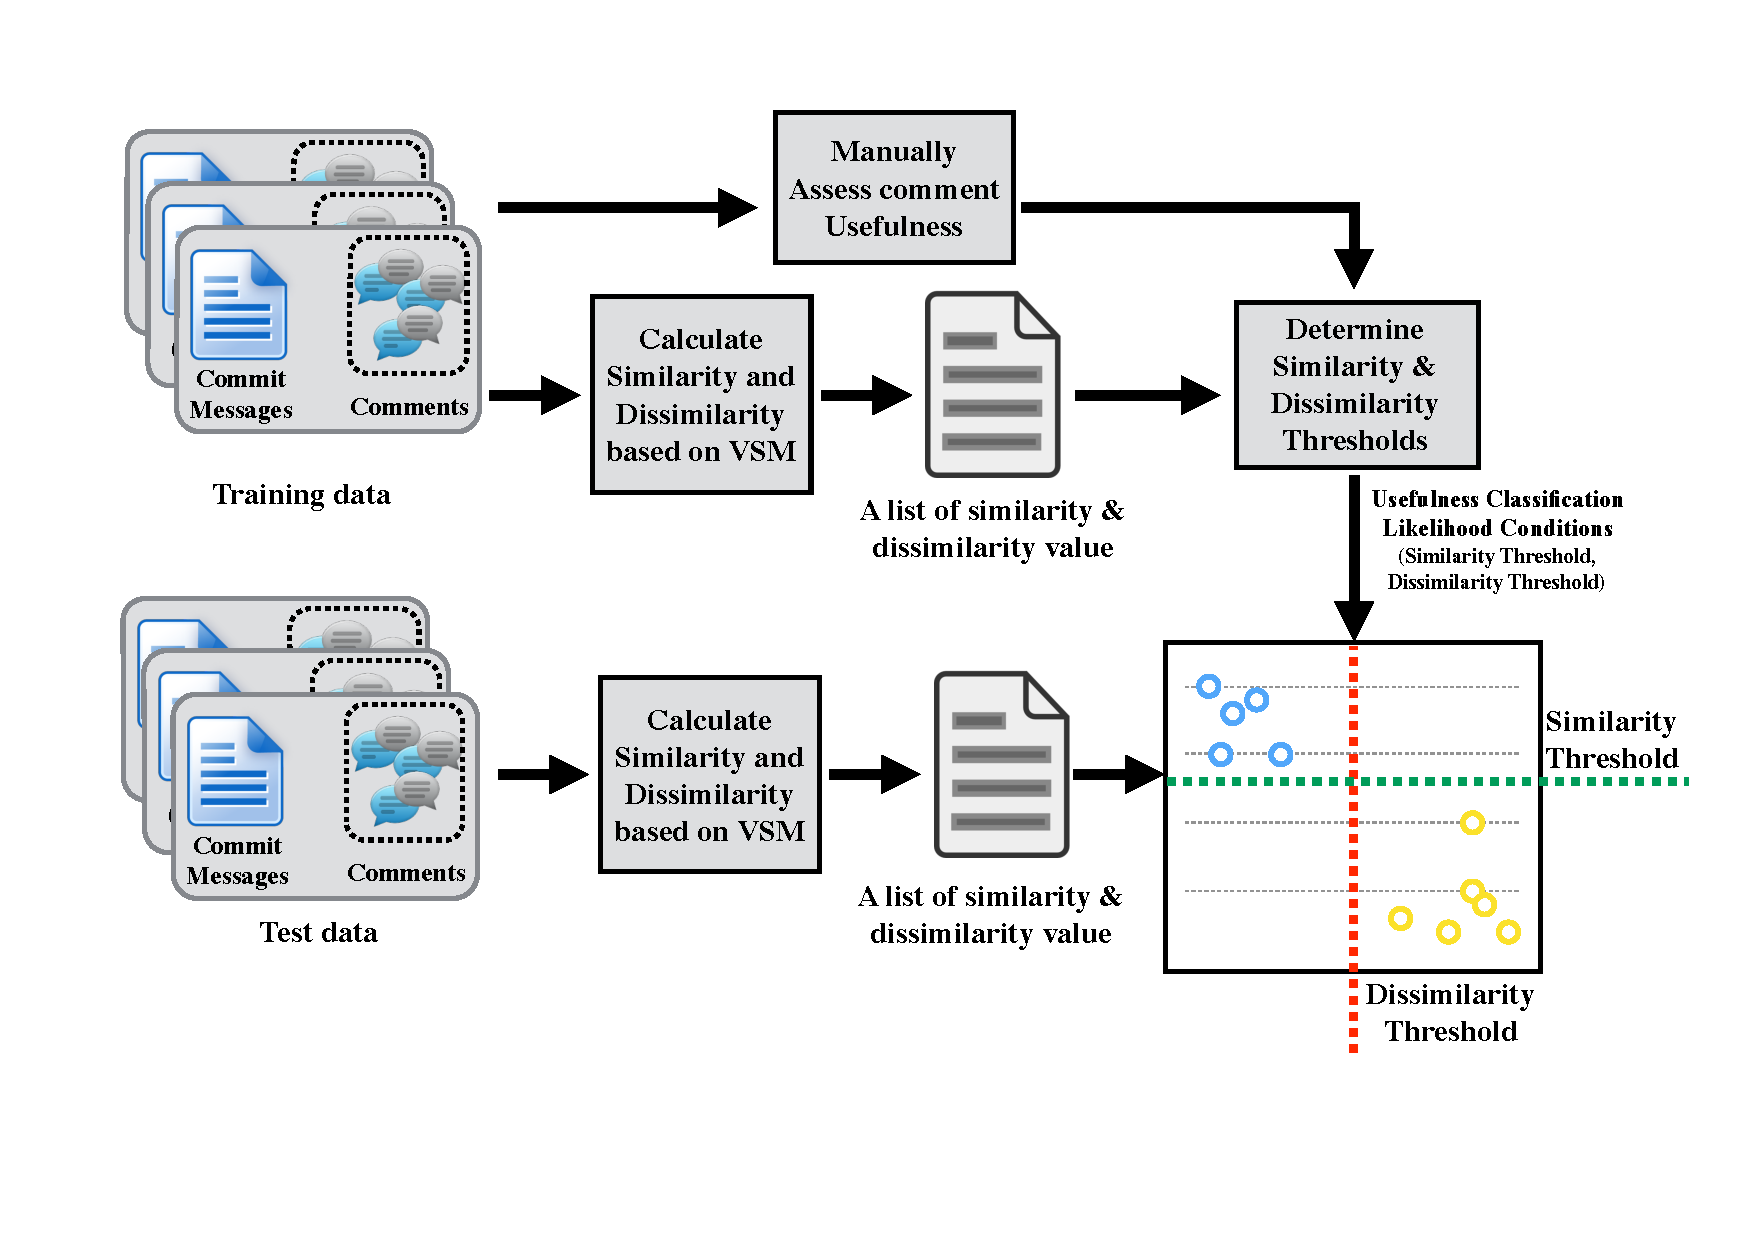
\includegraphics[scale=0.34, trim = 50 90 0 30, clip=true]{overview2}
\caption{Overview of our classification approach.}
\label{fig:overview}
\end{figure}

Our goal is to improve the efficiency and confidence in determining the usefulness of review comments.
As discussed previously, this is largely based on relevance the comment has to the proposed change (as documented within a MCR system).
According to relevance theory, a primary factor in relevance is similarly, and so it is natural for us to consider classification using \emph{similarity conditions}. 
\dan{can we find a reference for relevance and similarly?}

That is, we assume that that the more similar a comment is to the proposed change, the more relevant it is and hence more likely useful.
Conversely, the more dissimilar\footnote{This can be arbitrarily large, thus not simply the opposite of similarity.}, the less relevant, and hence less useful.

Given the subjective nature of usefulness, precise classification conditions probably do not exist and so we resort to conditions that indicate a meaningful \emph{likelihood} of classification.
That is, for some degree of similarity a comment is most likely useful, and for some degree of dissimilarity it is most likely not useful.
The key is determining these degrees in a practical and effective manner.

Fig. \ref{fig:overview} shows an overview of our proposed classification approach.
Usefulness of a comment is determined by computing its semantic similarity with the commit message of proposed change and observing if it satisfies \emph{usefulness classification likelihood conditions}.
The conditions are simply threshold values of similarity and dissimilarity empirically determined to optimize a desired likelihood objectives.
In our case example we chose to maximize the F-measure, but other likelihood functions could be used depending on precision, recall, or risk goals.

% again, I can't see Fig. \ref{fig:overview}(a)
% Thai sez: Cosine distance IS NOT cosine similarity. Cosine distance is defined as 1 - cosine similarity, and is not a proper distance metric, lacking triangle equality and stuff [Wikipedia].
To calculate semantic similarity, we used the Vector Space Model (VSM) with the cosine similarity measure, which is a well-known technique for retrieving similar documents written in unstructured natural language; and the Euclidian distance, which is a well-established measure of dissimilarity and applies analogously.
%For our case example training dataset, we manually identified 320 randomly-selected pairs of comments and corresponding commit messages in Fig. \ref{fig:overview}(b). \thai{The %overview figure does not have (a) and (b)...}
%\dan{what was the actual effort (in person-hours) to create the training data?}

Our training data is a small set of randomly-selected pairs of comments and the corresponding commit messages.
These comments are manually assessed for usefulness.
Each comment is assessed by three different people independently.
For each \texttt{YES} vote, a single point is given to that comment.
This means that a comment will receive a score of 0, 1, 2, or 3.
For statistical purposes, at least 30 useful and 30 useless comments must be collected.

The similarity and dissimilarity metrics are then computed for the data set.
These are used to estimate the similarity and dissimilarity thresholds $S_T$ and $D_T$ that can best (relative to some likelihood function such as F-measure) discriminate useful comments and $S'_T$ and $D'_T$ for useless comments.

Using these thresholds, we can classify the usefulness of comments for the rest of comments in review history according to the classification model as follows: given a comment $c$ and a corresponding commit message $m$,
\begin{itemize}
\item \textbf{useful}: $\Theta(c,m,S_T,D_T) = \True$ iff $\Sim(m,c) \geq S_T$ and $\Dist(m,c) \leq D_T$.
\item \textbf{useless}: $\Omega(c,m,S'_T,D'_T) = \True$ iff $\Sim(m,c) \leq  S'_T$ and $\Dist(m,c) \geq D'_T$.
\item \textbf{undetermined}: neither or both of the above conditions are $\True$.
% We also refer to them as \emph{neither} and \emph{overlap}.
\end{itemize}

The functions $\Sim(m,c)$ and $\Dist(m,c)$ are the similarity and dissimilarity measures relative to the proposed change commit message $m$ for the text of comment $c$.
Two metrics are used because they are independently generated and thus provides better discrimination for classification.
We also found experimentally that using two metrics has higher performance than just one. 

% The details of our approach are elaborated in the following subsections.

%\dan{**** ALERT **** this entire subsection is not needed! Everything in it is well-known and can simply be referenced. I suggest removing it if we need the space.  I have not edited this section .... }
%\subsection{Similarity and Dissimilarity Calculation based on VSM}
%%Vector Space Model (VSM) is well-known technique for information retrieval where documents written in unstructured natural language. In Software Engineering, VSM has been widely use to find relationship among documents in software issue tracking system\cite{Davies2012}.
%For each review, we compute similarity and dissimilarity of every comments comparing with the commit message which is described the purpose of the change.
%To do so, we use VSM which is a model for representing text documents as vectors.
%For a set of commit messages and comments ($D$), each document, $d$ (commit message or comment) is represented as $\overrightarrow{V_d} = <w_{1,d},w_{2,d},w_{3,d},...w_{n,d}>$, where $n$ is the total number of unique terms occur in $D$.
%The $w_{t,d}$ value is tf-idf weighting of term $t$ calculated from term occurrence frequency using Equation \ref{eq:tf-idf} where $\operatorname{tf}_{t,d}$ is frequency of term $t$ occurs in document $d$; and $|\{d' \in D | t \in d'\}|$ is the number of other documents $d'$ that also contain term $t$.  
%
%\begin{equation}
%w_{t,d} = \operatorname{tf}_{t,d} \times \log\frac{|D|}{|\{d' \in D \:|\: t \in d'\}|}
%\label{eq:tf-idf}
%\end{equation}
%
%After transforming commit message and comments to vectors, we calculate similarity using Cosine similarity and Euclidian distance. 
%
%
%\noindent\textbf{Cosine similarity} measures similarity between two vectors using inner product. Given a vector commit message $\overrightarrow{V_m}$ and the vector of its comments $\overrightarrow{V_m}$, we can calculate Cosine similarity using Equation \ref{eq:cosine}. The similarity value is ranging $[0,1]$ where 0 means there is no similarity and 1 means two vectors are textually similar.  
%
%\begin{equation}
%\Sim(c) = \cos\theta(\overrightarrow{V_m},\overrightarrow{V_c}) = \frac{\sum_{i=1}^{|D|} w_{i,m} \times w_{i,c}}{\sqrt{\sum_{i=1}^{|D|} w^2_{i,m} \times \sum_{i=1}^{|D|} w^2_{i,c}}}
%\label{eq:cosine}
%\end{equation}
%
%\noindent\textbf{Euclidian distance} measures ordinary distance between each element of two vectors using Equation \ref{eq:euclid}. We can use this distance as an dissimilarity. Given a vector commit message $\overrightarrow{V_m}$ and the vector of its comments $\overrightarrow{V_m}$, we can calculate Euclidian distance using Equation \ref{eq:cosine}. The distance value is ranging $[0,\infty)$ where 0 means these vectors are the same vectors while a more distance means these vectors are less similar.
%
%\begin{equation}
%\Dist(m,c) = \|\overrightarrow{V_m} - \overrightarrow{V_c}\| = \sqrt{\sum_{i=1}^{|D|}(w_{i,m} - w_{i,c})^2}
%\label{eq:euclid}
%\end{equation}
%
%\subsection{Estimating Similarity and Dissimilarity Thresholds}
%Suppose we use $\Theta(c,S_T=s_t,D_T=d_t)$ to classify useful comments and we have the following values:
%
%$\mathrm{TP}_{s_t,d_t}$ is the number of comments that our model classified as \textit{useful} and are \textit{actually useful} i.e. true-positives; 
%
%$\mathrm{FP}_{s_t,d_t}$ is the number of comments that our model classified as \textit{useful} but are \textit{actually useless} i.e. false positives;
%
%$\mathrm{FN}_{\theta_s,\theta_d}$ is the number of comments that our model classifies as \textit{useless} but are \textit{actually useful}. 
% 
%We can now define the following classification  performance measures: 
%\begin{equation}
%\begin{split}
%\mathrm{F\text{-}measure}_{s_t,d_t} &= 2 \times \frac{\mathrm{precision}_{s_t,d_t} \times \mathrm{recall}_{s_t,d_t}}{\mathrm{precision}_{s_t,d_t} + \mathrm{recall}_{s_t,d_t}}
%\\
%\mathrm{precision}_{s_t,d_t}  &= \frac{\mathrm{TP}_{s_t,d_t}}{\mathrm{TP}_{s_t,d_t}+\mathrm{FP}_{s_t,d_t}}
%\\
%\mathrm{recall}_{s_t,d_t}  &= \frac{\mathrm{TP}_{s_t,d_t}}{\mathrm{TP}_{s_t,d_t}+\mathrm{FN}_{s_t,d_t}}
%\end{split}
%\label{eq:fmeasure}
%\end{equation}

We find similarity and dissimilarity thresholds by selecting $s_t,d_t$ values that maximize the F-measure,
which is a performance measure for a binary classification that compromises trade-offs in accuracy of classification (precision) and coverage of classification (recall).
In this paper, we used the F$_1$ measure, which gives equal weight to both precision and recall.
Depending on application, different weights can be given by choosing a different F$_\beta$ measure.

% Our proposed approach is empirically driven and automatically adjusts to the quality the data.
While our proposed approach is straightforward, empirically driven, and automatically adjusts to the quality of the data, it has a few drawbacks.
First, we have to accept that some comments cannot be reliably or confidently classified.
We denote these as \emph{undetermined} to differentiate them from comments whose usefulness is \emph{unclear} (i.e. cannot be assessed subjectively).
Secondly, owing to the subjective assessment of usefulness, this representation fundamentally implies supervised classification requiring nontrivial training data to define representative classification sets.
This decreases the cost-effectiveness and limits the practicality of application to projects with a large enough number of comments, where the classification effort saved overcomes the training costs.  
% empirically driven and automatically adapts to the quality the data


% Thai sez: We did not mention the F-measure for \Theta, thus suddenly referring to \Omega does not make much sense...
% The F-measure for $\Omega(c,S_T=s_t,D_T=d_t)$ is computed analogously where we change instances of useful to useless and vice-versa in the definitions. The correctness of classification is determined from the useful/useless defined dataset. 


%Using this method, we iteratively measure an accuracy for values of $s_t$ and $s'_t$ ranging $[0,1]$; and values of $d_t$ and $d'_t$ ranging $[0,\infty)$. 

%\begin{equation}
%\mathrm{F\text{-}measure}_{S_T,D_T} = \frac{2\mathrm{TP}_{S_T,D_T}}{2\mathrm{TP}_{S_T,D_T}+\mathrm{FP}_{S_T,D_T}+\mathrm{FN}_{S_T,D_T}}
%\label{eq:precision}
%\end{equation}

%where $\mathrm{TP}_{S_T,D_T}= |\{ c \in C |  \text{\textbf{useful}}(c,S_T,D_T) = \mathrm{TRUE} \}\cap \{c \in C| \mathrm{vote}(c) = 2\}|$,  $\mathrm{FP}_{S_T,D_T} = |\{ c \in C | \text{\textbf{useful}}(c,S_T,D_T) = \mathrm{FALSE} \}\cap \{\mathrm{vote}(c) = 2\} $, $\mathrm{FN}_{S_T,D_T} = |\{ c | c \in C, \text{\textbf{useful}}(c,S_T,D_T) = \mathrm{TRUE} \}\cap \{\mathrm{vote}(c) < 2\} $
%According to this, we can formalize as follows:

%\begin{equation}
%(S_T,D_T) = \max(\{\mathrm{F\text{-}measure} \text{ of \textbf{useful}}(c,s_T,d_T) | s_T\in[0,1] \text{ and } d_T\in [0,\infty) \})
%\end{equation}
